\chapter{Comparação das métricas por modelo e \textit{dataset}}
\label{apen:a}

\begin{figure}[!htp]
    \centering
    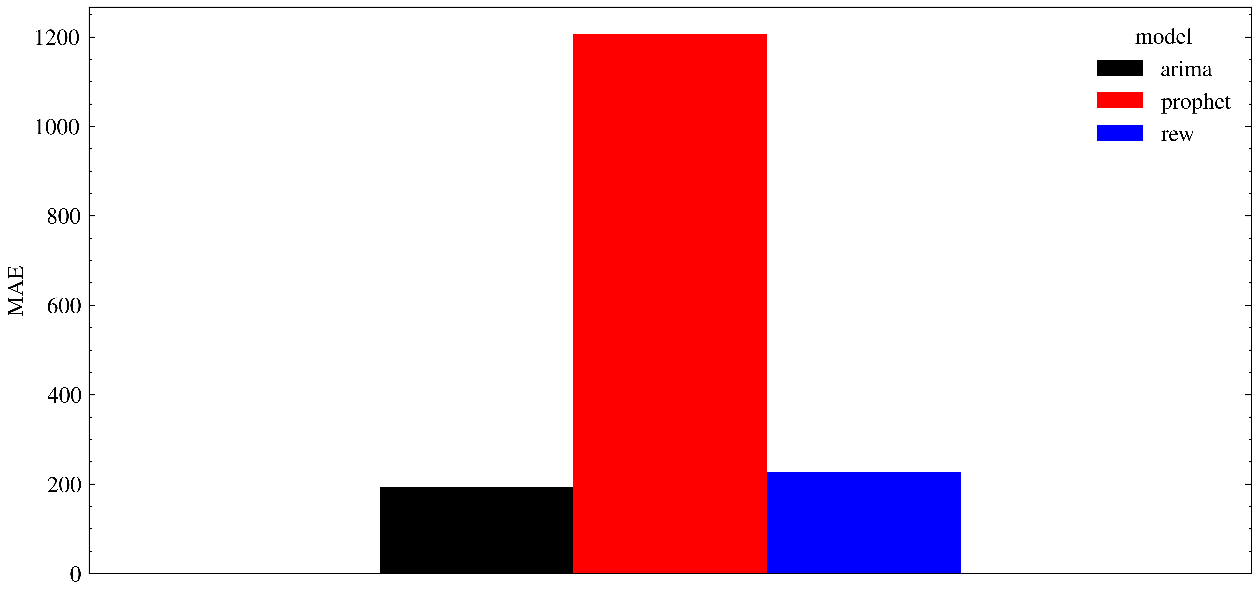
\includegraphics[width=5.0in]{img/covid_mae_comparison.pdf}
    \caption{MAE por modelo para o número de casos confirmados de Covid-19.}
\end{figure}

\begin{figure}[!htp]
    \centering
    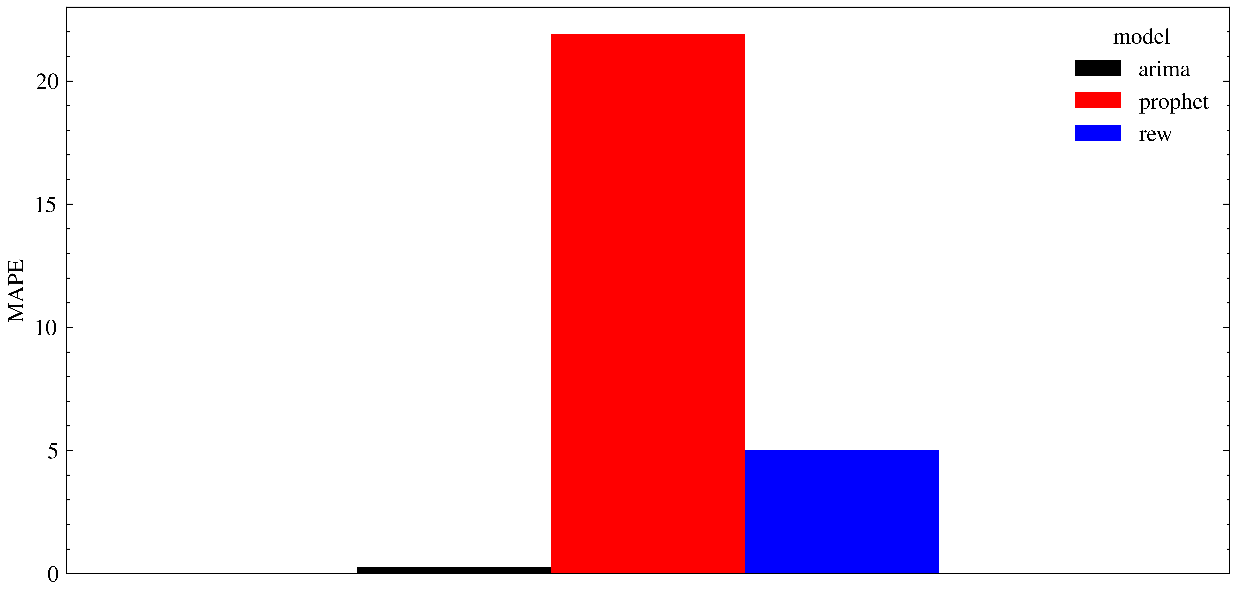
\includegraphics[width=5.0in]{img/covid_mape_comparison.pdf}
    \caption{MAPE por modelo para o número de casos confirmados de Covid-19.}
\end{figure}

\begin{figure}[!htp]
    \centering
    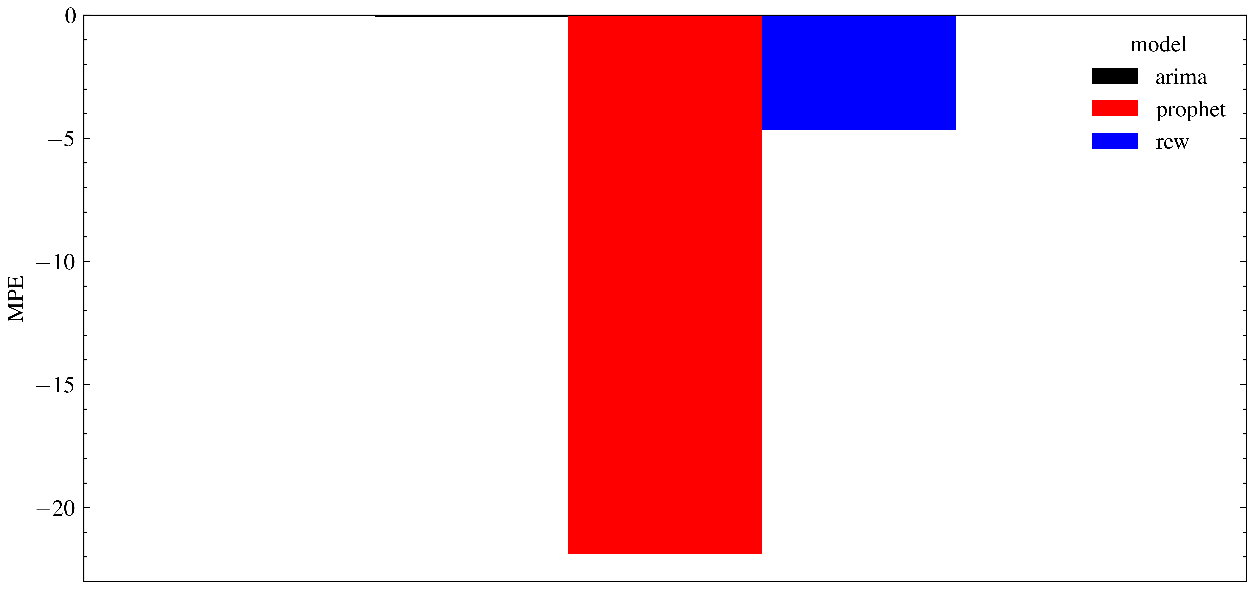
\includegraphics[width=5.0in]{img/covid_mpe_comparison.pdf}
    \caption{MPE por modelo para o número de casos confirmados de Covid-19.}
\end{figure}

\begin{figure}[!htp]
    \centering
    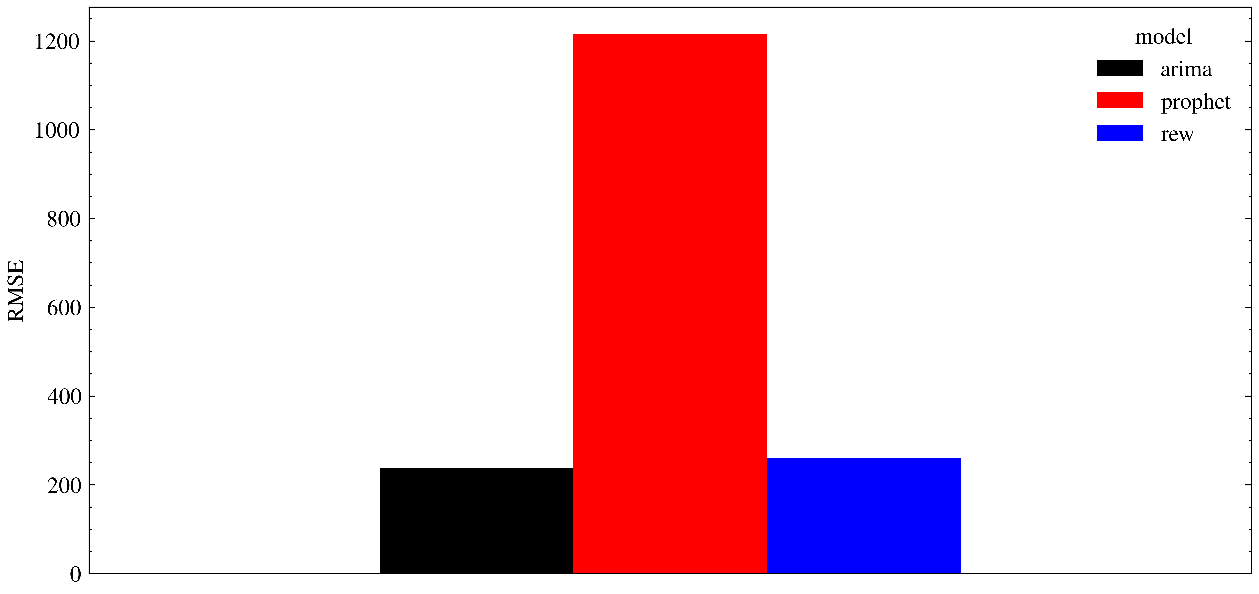
\includegraphics[width=5.0in]{img/covid_rmse_comparison.pdf}
    \caption{RMSE por modelo para o número de casos confirmados de Covid-19.}
\end{figure}

\begin{figure}[!htp]
    \centering
    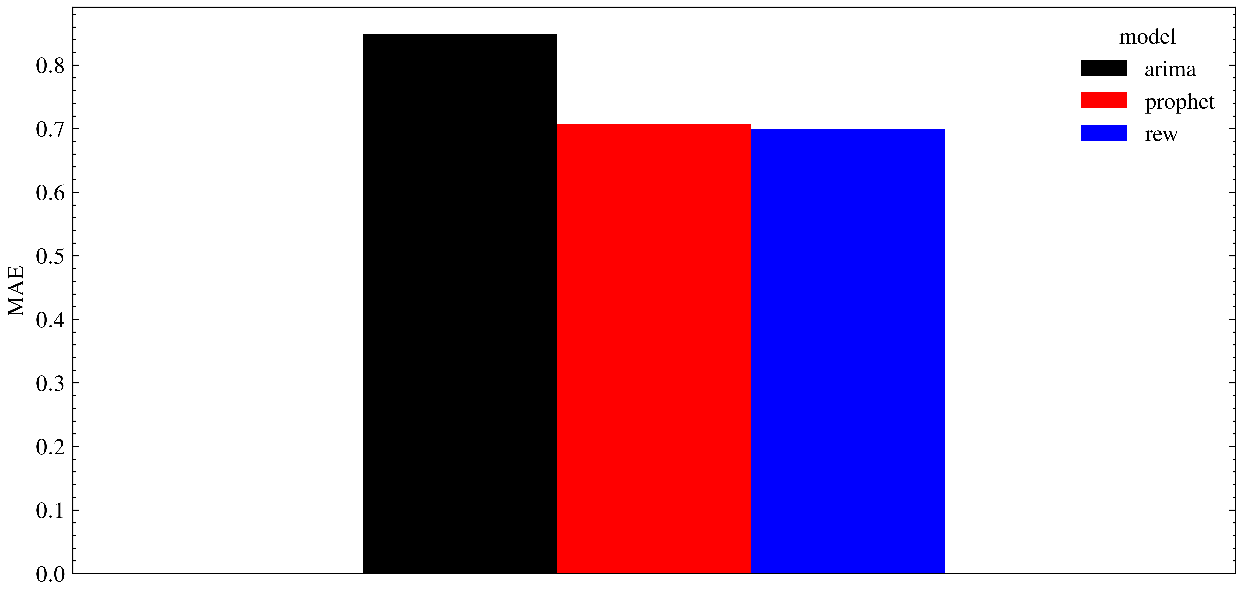
\includegraphics[width=5.0in]{img/temperatures_mae_comparison.pdf}
    \caption{MAE por modelo para a temperatura diária de Melbourne.}
\end{figure}

\begin{figure}[!htp]
    \centering
    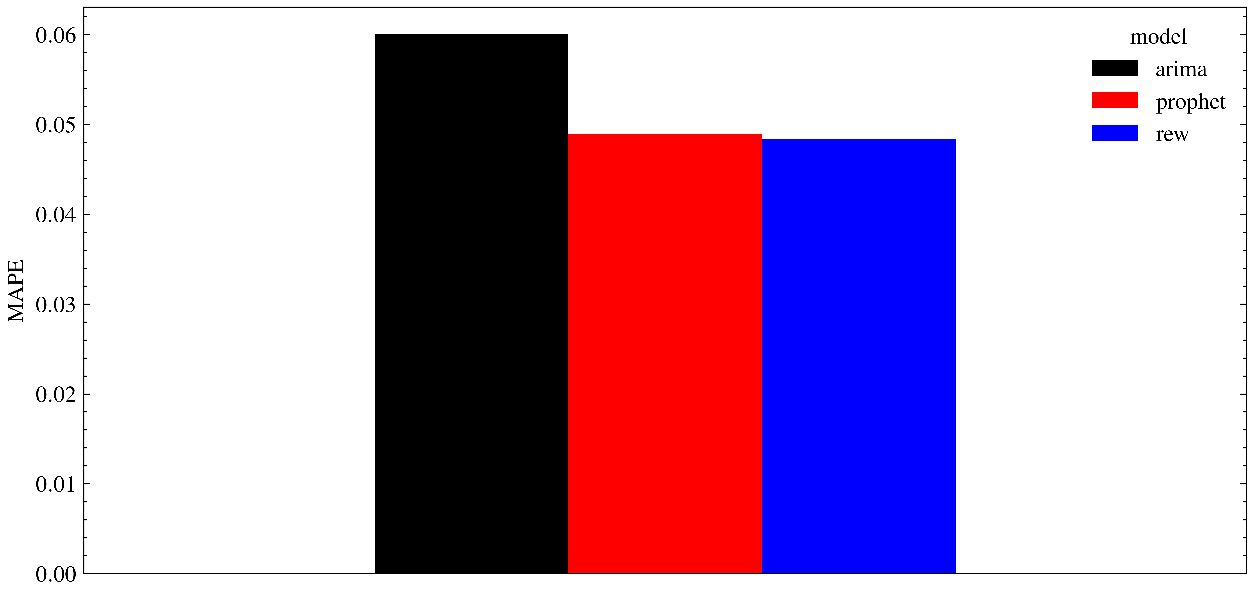
\includegraphics[width=5.0in]{img/temperatures_mape_comparison.pdf}
    \caption{MAPE por modelo para a temperatura diária de Melbourne}
\end{figure}

\begin{figure}[!htp]
    \centering
    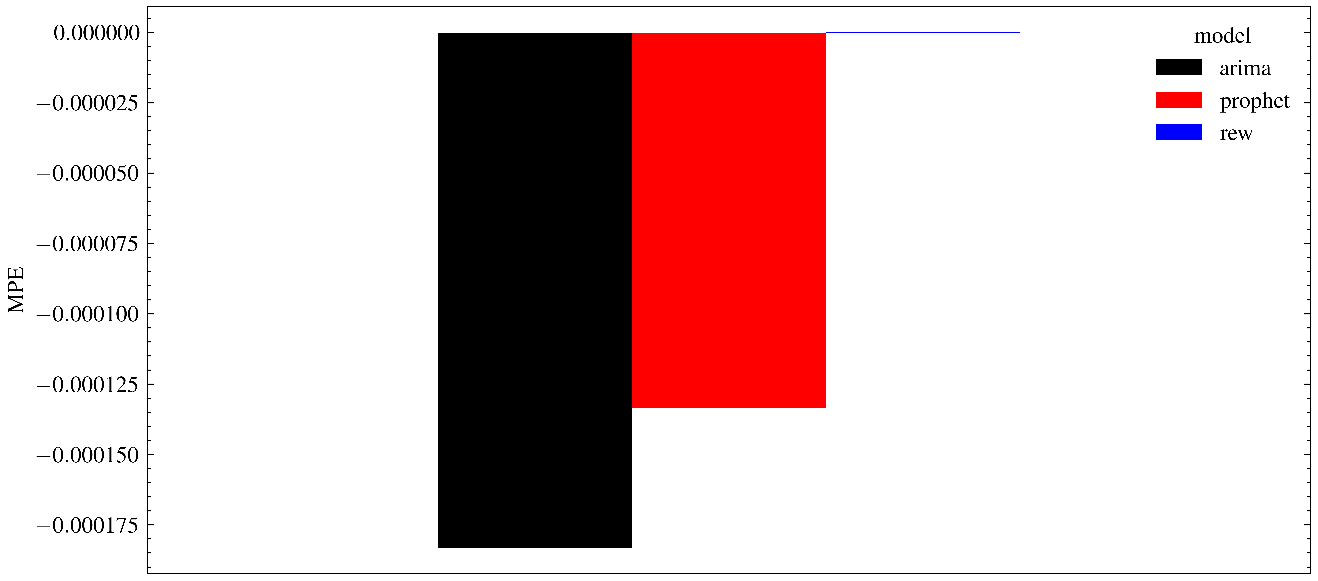
\includegraphics[width=5.0in]{img/temperatures_mpe_comparison.pdf}
    \caption{MPE por modelo para a temperatura diária de Melbourne}
\end{figure}

\begin{figure}[!htp]
    \centering
    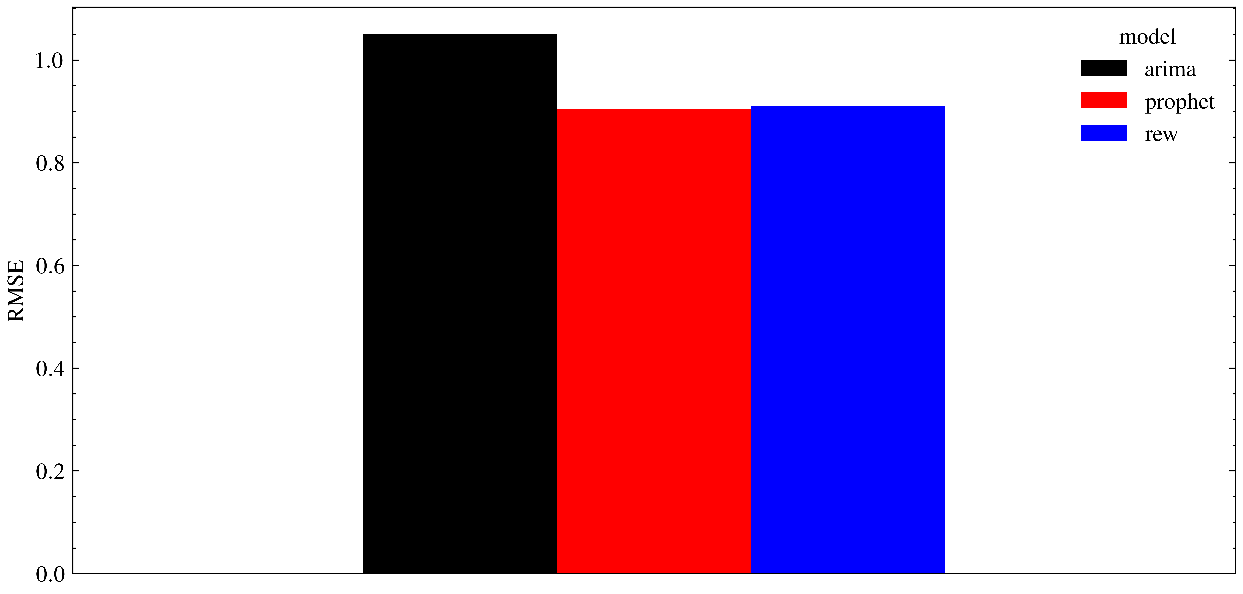
\includegraphics[width=5.0in]{img/temperatures_rmse_comparison.pdf}
    \caption{RMSE por modelo para a temperatura diária de Melbourne}
\end{figure}

\begin{figure}[!htp]
    \centering
    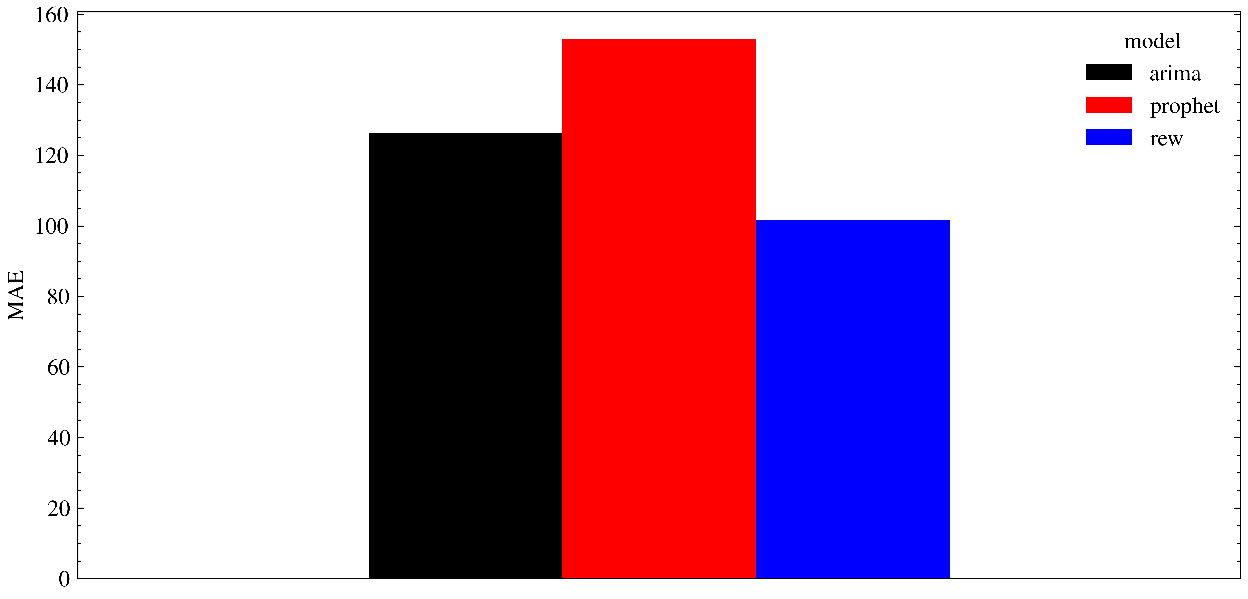
\includegraphics[width=5.0in]{img/synthetic_mae_comparison.pdf}
    \caption{MAE por modelo para os dados sintéticos.}
\end{figure}

\begin{figure}[!htp]
    \centering
    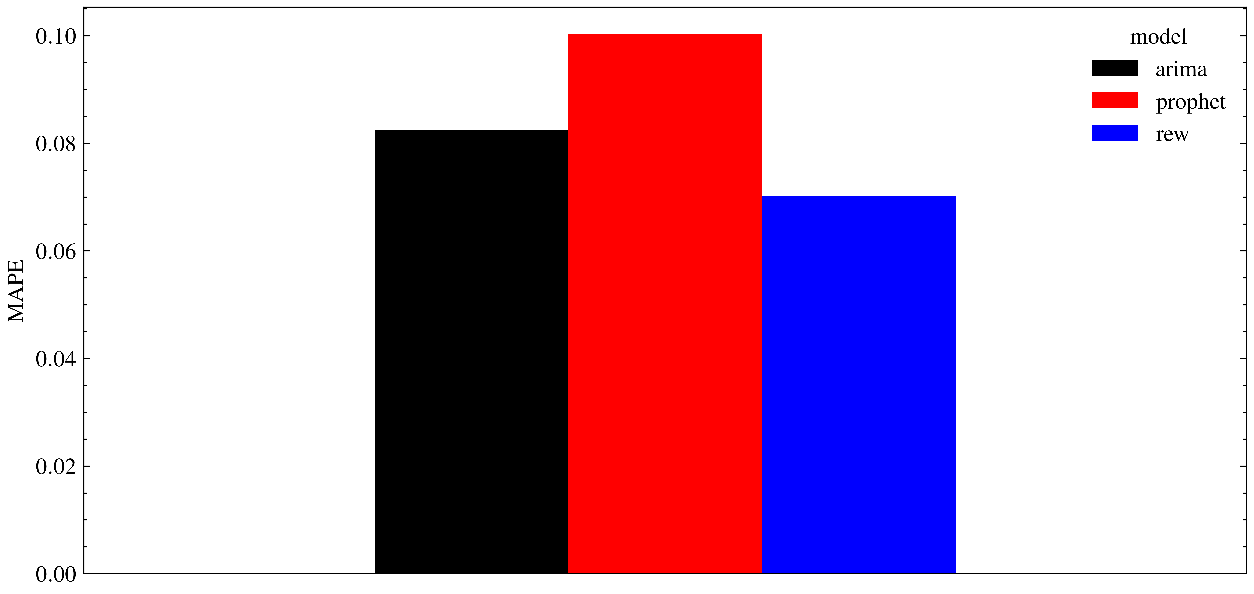
\includegraphics[width=5.0in]{img/synthetic_mape_comparison.pdf}
    \caption{MAPE por modelo para os dados sintéticos.}
\end{figure}

\begin{figure}[!htp]
    \centering
    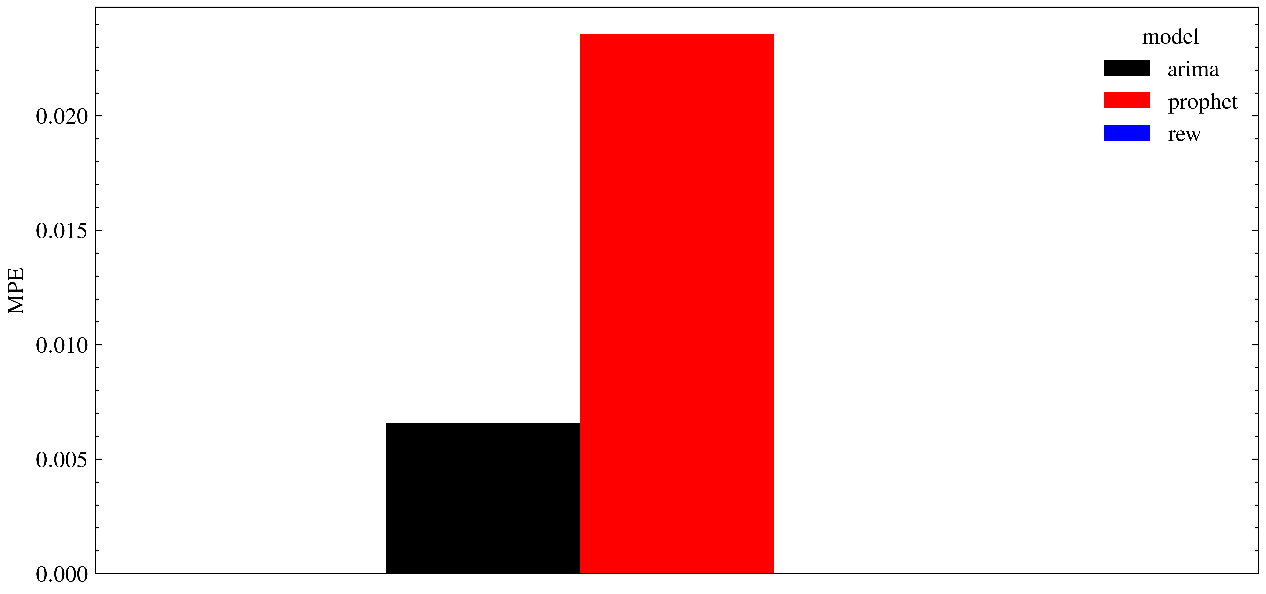
\includegraphics[width=5.0in]{img/synthetic_mpe_comparison.pdf}
    \caption{MPE por modelo para os dados sintéticos.}
\end{figure}

\begin{figure}[!htp]
    \centering
    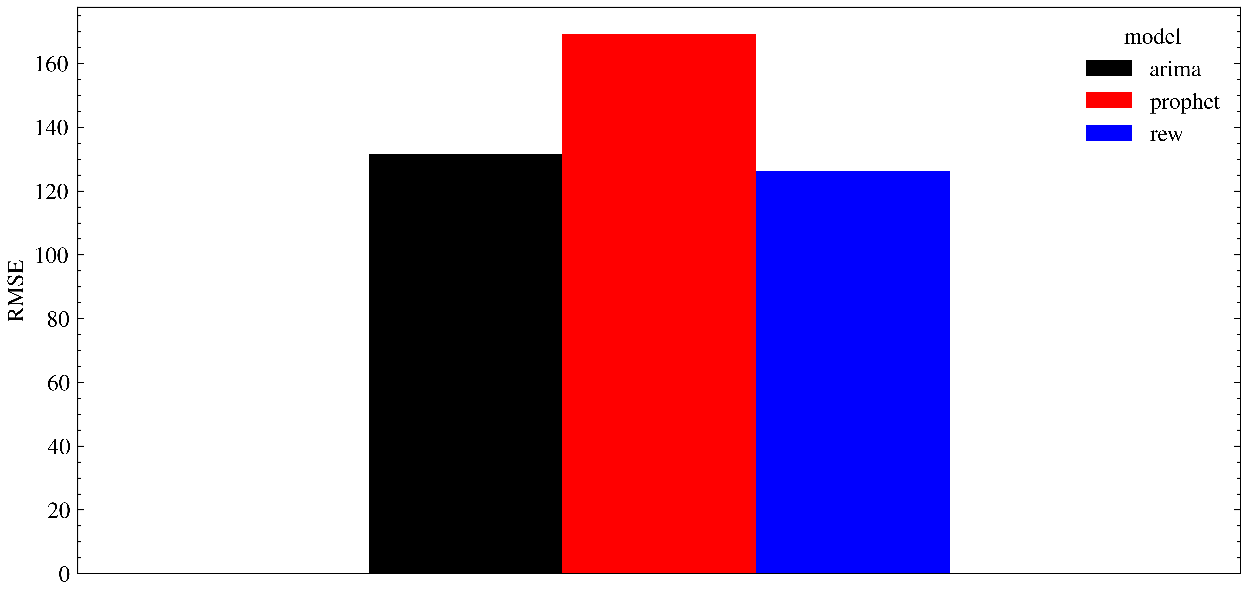
\includegraphics[width=5.0in]{img/synthetic_rmse_comparison.pdf}
    \caption{RMSE por modelo para os dados sintéticos.}
\end{figure}
